\documentclass[tikz,border=15pt]{standalone}
\usepackage{circuitikz}
% [2026-08-03 KNOT DISAMBIGUATION per manuscript/ave-kb/CLAUDE.md:22 INVARIANT-N1
%  (knot / trefoil disambiguation clause), verbatim: "the electron's **real-space body** is the
%  $0_1$ **unknot**; the proton's is the $6^3_2$ **Borromean** linkage. Rolfsen names ($3_1$
%  trefoil, $5_1$ cinquefoil, ...) and '$(2,q)$ torus knot' labels refer to **phase-space winding
%  portraits** on the bond-pair LC tank (Clifford torus), **not** real-space body knots. Never
%  write 'trefoil electron' without an explicit *phase-space* qualifier; valence electrons in
%  orbital topology are $0_1$ unknot solitons on harmonic tracks."
%  The orbital node label below carried a bare Rolfsen $3_1$ on the hydrogen VALENCE ELECTRON --
%  the exact case the invariant's last clause names. Prior wording (git trail):
%  "Orbital Phase Tank ($3_1$)".
%  It also contradicted its own consuming chapter: chapters/03_hydrogen.tex:52 already prints
%  "orbited by the electron's $0_1$ unknot flux tube (carrying the canonical $(2,3)$ phase-space
%  Clifford-torus winding ...)". Rewritten to that form -- same pattern as the merged vol6 twin
%  (#852, figures/circuit_h3_decay.tex) and the vol4 pilot (#843,
%  14_particle_decay_spice.tex:94 figure caption).
%  UNTOUCHED and CORRECT: the $6^3_2$ label on the Nucleon Tank -- INVARIANT-N1 names the $6^3_2$
%  Borromean linkage as the proton's REAL-SPACE body. No circuit element, coupling or geometry
%  is changed.
%  GENERATOR: this file is emitted by src/scripts/vol_6_periodic_table/circuits/make_circuits.py
%  (tex_h1 string); that source carries the same correction so a regeneration cannot revert it.]
\begin{document}
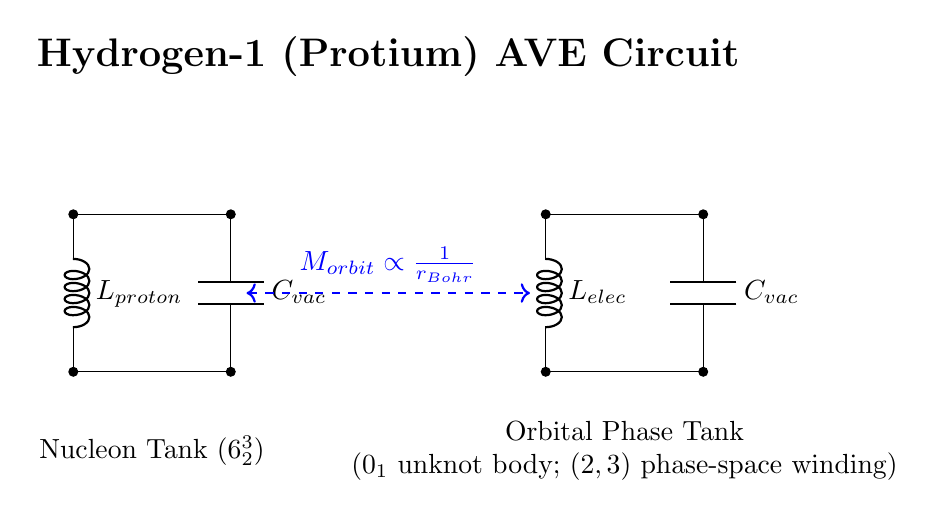
\begin{tikzpicture}
    \begin{scope}[shift={(0,0)}]
        \draw (0,0.5) to[L=$L_{proton}$, *-*] (0,-1.5);
        \draw (2,0.5) to[C=$C_{vac}$, *-*] (2,-1.5);
        \draw (0,0.5) -- (2,0.5);
        \draw (0,-1.5) -- (2,-1.5);
        \node at (1, -2.5) {Nucleon Tank ($6^3_2$)};
    \end{scope}

    \begin{scope}[shift={(6,0)}]
        \draw (0,0.5) to[L=$L_{elec}$, *-*] (0,-1.5);
        \draw (2,0.5) to[C=$C_{vac}$, *-*] (2,-1.5);
        \draw (0,0.5) -- (2,0.5);
        \draw (0,-1.5) -- (2,-1.5);
        \node[align=center] at (1, -2.5) {Orbital Phase Tank\\($0_1$ unknot body; $(2,3)$ phase-space winding)};
    \end{scope}

    \draw[<->, dashed, blue, thick] (2.2,-0.5) -- (5.8,-0.5) node[midway, above] {$M_{orbit} \propto \frac{1}{r_{Bohr}}$};

    \node at (4, 2.5) {\Large \textbf{Hydrogen-1 (Protium) AVE Circuit}};
\end{tikzpicture}
\end{document}
